\section{Experiments}
\label{sect:experiments}
\subsection{Introduction}
The simulation experiments are performed using schedulers built with the Scheduler Component Architecture (SCA) described in (Sect.~\ref{sect:architecture}). In order to setup a specific simulation experiment it is necessary to devise both a scheduler implementation and a simulation experiment control application (SEC\glossary{name={SEC},description={Simulation Experiment Controller - a control application specific to a simulation experiment}}) specific to the experiment (or set of experiments). Fig.~\ref{fig:sim_frame_arch} shows the general architecture of a typical simulation experiment. The SEC creates the various data models (Phase2, accounting, history, environment, etc) and resource tools (execution timing calculator, environment prediction, etc) and makes these available to the scheduler via the simulation engine (simulator). The simulator's operating cycle involves making scheduling requests, performing these and notifying the SEC. The SEC is then responsible for collation of any relevant statistics.


\begin{figure}[htbp]  
  \begin{center}
    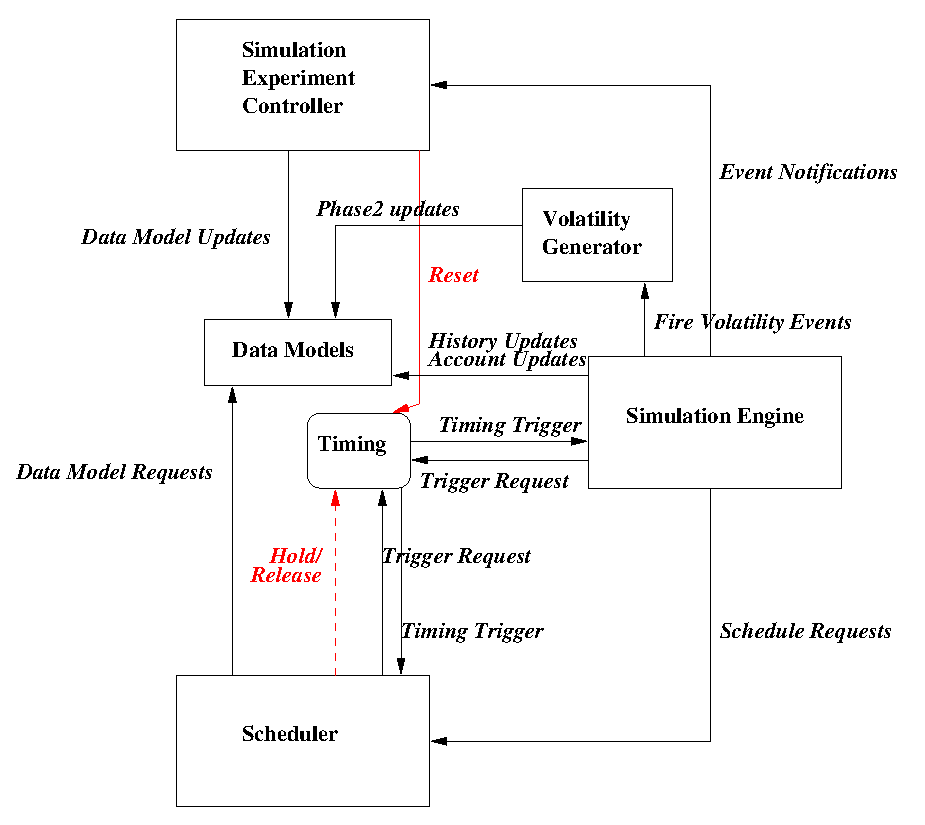
\includegraphics[scale=0.8, angle=0]{figures/sim_framework_arch.eps}
  \end{center}
  \caption[The simulation architecture.]
   {The simulation architecture. The Simulation Experiment Control application (SEC) is responsible for creating the various data models used by the scheduler. It invokes the simulator to run between specified times and receives feedback of significant scheduling events. The simulator makes scheduling requests of the scheduler and provides updates to the data models when the observations are deemed to have completed. Synchronization between components in speeded up simulation time is provided by the Time Signal Generator (TSG).}
  \label{fig:sim_frame_arch}
\end{figure}

The general format of a nights observing is in the form of a series of events. After each group has started executing there is generally nothing of significance capable of occuring from a scheduling point of view until the group completes or fails. To take advantage of this, the simulator is designed to operate by generation of discrete events. It had been anticipated that the time used in the model could simply be set to run at the maximum possible as permitted by the cycle of $schedule -> execute -> update$.

 However, because certain component operations within scheduler implementations might have to run as seperate threads (in the real world), there would have to be a form of time synchronization to allow these types of component to work correctly in the speeded up simulation environment. To illustrate by an example:

 A specific scheduler implementation might be required to run a sorting operation which takes perhaps 2 seconds of real time (a long time by simulation standards) every 5 minutes. Now 2 seconds of real time might actually correspond to several minutes or hours of simulation time, resulting in the sorting operation going \emph{out of phase} with the rest of the simulation. 

 This was solved by creating a Timing Signal Generator (TSG). This component permits several operations. In the main, an external client may request an asynchronous time-trigger at some future (simulation) time. The TSG keeps track of trigger requests and sends these signals out asynchronously to the requestors, in order, at the appropriate (simulation) times. Additionally, any client (thread) which requires to perform a \emph{significant} real-time operation may place a hold on the TSG to prevent any triggers being emitted. After completion of the real-time operation the client releases the hold and any queued triggers can be sent out. Ultimately, provided there are no extremely time-hungry real-time operations, the simulation clock advances significantly faster than real-time.

\subsection{Simulator Operation}
\label{ss:sim_ops}
The operation of the simulator cycle is described in Fig.~\ref{fig:ss_vgen_flowchart}. The simulator is controlled by an SEC and on initiation runs for a period specified by the SEC. With reference to the figure, a cycle of $schedule->execute->update$ is performed. Initially the simulation time $t$ is set to the start time specified by the SEC. A series of tests are then performed to determine \emph{what to do next} and \emph{how long} (denoted $\tau$) this operation will take in terms of simulation time. 

The first test determines if $t$ is during daytime. If so the simulation will skip forward to the calculated sunset time. If not, the second test determines if $t$ occurs during any scheduled \emph{disruptive} event (bad weather, mechanism failure, engineering time). If so the time will be advanced to the end of this disruption. If not, an observation group is requested from the schedule despatcher. If none are available, the simulation will skip forward by the length of a \emph{background observation} (effectively idle time). If a group is returned from the despatcher, the \emph{expected} execution time $\tau_{exec}$ is determined and a further test is performed to determine of any disruptive events are scheduled to start between $t$ and $t+\tau_{exec}$. If not, the simulation will be advanced to $t+\tau_{exec}$, otherwise to the start of the disruption $t+\tau_{sod}$. 

Once the advance ($\tau$) has been determined, but before the time is actually incremented, it is guaranteed that nothing can occur in this interval to affect the run of the simulation. At this point the Volatility Generator is called upon to effect any Phase 2 update events scheduled for the period $[t, t+\tau]$. The simulation time is then advanced by the relevant amount. If a group has been selected for execution it will have either succeeded or failed (it may have been aborted by a disruption event). The various models (history, accounting) are then updated and the SEC receives a notification from the simulator of group completion (or failure).


\begin{figure}[htbp]
\begin{center}
    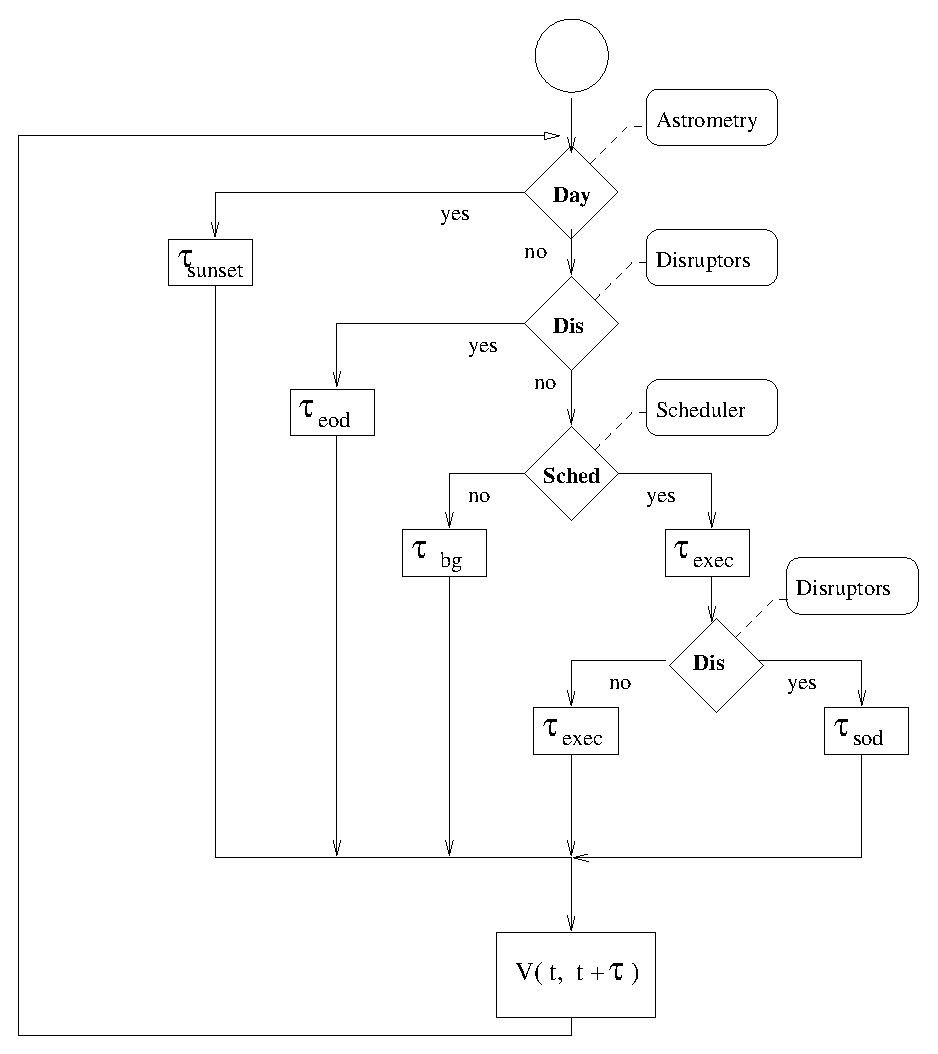
\includegraphics[scale=1.0, angle=0]{figures/ss_algorithm.eps}
\end{center}
\caption[Flowchart for simulation algorithm.]
{Flowchart for simulation algorithm. The time advance values are: $\tau_{ss}$ time-until-sunset; $\tau_{eod}$ time until end of current disruption event; $\tau_{sod}$ time until start of next disruption event; $\tau_{bg}$ background observing time; $\tau_{exec}$ execution time of a group. The decision boxes represent the following tests:- \begin{inparaenum} [(\itshape i\upshape)] \item $Day(t)$ - is time $t$ daytime ?, \item $Dis(t)$ - is time $t$ inside some disruption period ?, \item $Sched(t)$ - can the despatcher find anything to do at $t$ ?, \item $Dis(t, t+\tau)$ - are there any disruption events starting during the interval $(t, t+\tau)$. \end{inparaenum}.}
\label{fig:ss_vgen_flowchart}
\end{figure}


\subsection{Sources of uncertainty}
\label{sect:exp_uncertainty}
The real environment in which operational schedulers have to function provides many sources of uncertainty (Sect.~\ref{sect:env_components}). The simulation framework is intended to provide a controlled environment for the scheduler to run in but must provide a realistic degree of variation in these environmental variables. These sources of uncertainty affect both the complexity of the scheduling problem (in terms of complexity metrics) and the range of potential rewards possible (in terms of schedule quality metrics). The main stochastic inputs are:-

\begin{description}
\item [Stochastic execution model (S)] While the \emph{execution resource estimation model} (X) provides an estimate of the amount of time a group is expected to take. The various schedulers use this to decide when a group is likely to complete, however in reality a group might take more or less time due to various sources of uncertainty. The \emph{Stochastic execution model} allows the simulation framework to take these effects into account and introduces some variation in the simulated execution times of groups. This is generally implemented by using the prediction from X then adding some gaussian or white noise to simulate the effect of variable length telescope and instrument operations.

\item [Environmental model (E)] On an actual night the seeing and atmospheric extinction may vary over the full range and with a variety of timescales. This natural variation in the sky conditions are taken into account by the \emph{environmental model}.

\item [Phase 2 model (P)] The distribution of the generator parameters used to create the Phase 2 information will affect the evolution of a schedule during the night since the Phase 2 model is what determines the set of feasible groups available.

\item [Disruption model (D)] Interruptions of varying sizes and lengths due to (unpredictable) disruptive events affect the degree of success of schedules, this aspect is simulated using a \emph{disruption model}.

\item [Volatility model (V)] Evolution or volatility of the phase 2 database content is simulated using a \emph{volatility model} which allows new groups to be injected into the ODB at (controlled) random intervals thus affecting the contention and other parameters of the Phase 2 model.

\end{description}


\subsection{Scheduler implementations}
\label{ss:sched_impl}
Two different types of scheduler are used in the experiments. These take rather different views of the process.

\subsection{Despatch Scheduler}
Despatch schedulers take a local view of optimization. At any point in time they will try to select the group $g$ which has the highest \emph{differential} score $f_g$ and which best matches current conditions. The algorithm is particularly straightforward:-

\begin{enumerate} 
\item The \emph{ExecutionFeasibilityModel} is used to generate a candidate list of groups which satisfy their timing constraints and all of their observing constraints under the current environmental conditions.

\item Using the \emph{ScoringModel}, various metrics and differential scores are calculated for each candidate group. 

\item The \emph{SelectionModel} is used to analyse the candidate metrics and choose one of these groups to execute.
\end{enumerate}

The baseline implementation used for simulations is called \emph{Basic Despatch Scheduler} (BDS\glossary{name={BDS},description={Basic despatch Scheduler - a simple scheduler}}). This implementation is typically configured to use different versions of \emph{SelectionModel} and \emph{ScoringModel}. For most cases the selection model $\xi_{BEST}$ is employed - this selects the highest scoring candidate group. Various biased selection models are tested in Sect.~\ref{sect:ss_exptsetup}. The scoring model employed is a weighted sum of a number of standard metrics such that the differential score $f_g$ for a candidate group $g$ at time $t$ under environmental conditions $E$ is given by Eq.~(\ref{eq:weighted_score}):-

\begin{equation}
\label{eq:weighted_score}
f_g = \sum_{i} {w_i f_i(g,t,E)}
\end{equation}

The \emph{execution timing model} used by BDS has a configurable fixed duration estimate assigned to each type of observing sequence component (see Fig.~\ref{fig:group} in Sect.~\ref{sect:intro_background}) with the exception of exposures for which the duration is calculated using configurable, instrument-specific overheads. (See Table.~\ref{tab:exectime_factors} for more details.)


%  \breve{o} \vec{o}

\subsection{Look Ahead Scheduler}
%\newcommand{\echelon}{$\mathsf{\breve{e}chelon}$ }
%\newcommand{\echelons}{$\mathsf{\breve{e}chelons}$ }

%\newcommand{\echelon}{$\mathsf{sequence}$ }
%\newcommand{\echelons}{$\mathsf{sequences}$ }

\newcommand{\echelon}{sequence}
\newcommand{\echelons}{sequences}

The Look-Ahead Schedulers (LAS) try to increase the overall reward by optimizing over a period of time (global optimization). They have to make estimates of what is likely to happen in the future - both in terms of external conditions (stability, volatility, disruption) and the likely outcomes of their own actions (how likely are the selected groups to succeed, will they overrun). In the discussion to follow the term \echelon refers to the ordered sequence of groups to execute during a given horizon. A typical LAS implementation works as follows:-

\begin{enumerate}
\item The \emph{HorizonDeterminant}, using information about environmental stability, ODB volatility and disruption decides how long the \echelon horizon (H) should be. If the horizon is too short we risk losing potential reward. If H is too long, we risk breakages.

\item Using the \emph{SolutionGenerator}, a number of candidate \echelons are generated in which each group must satisfy the timing and observing constraints under the predicted conditions at its expected time of execution according to the \emph{ExecutionFeasibilityModel}.

\item The \emph{ScoringModel} and \emph{ExecutionTimingModel} are then used to calculate a potential reward ($F_S$) for each \echelon $S$. If an EFR policy  is in force (Sect.~\ref{sect:architecture}) this would be used, perhaps in conjunction with environment and volatility prediction, to calculate the discount rate ($\lambda$). The discounted total reward for the \echelon is calculated using Eq.~(\ref{eq:discountreward}):-
\begin{equation}
\label{eq:discountreward}
F_S = \sum_{g \in S}{X_g f_g(t_g,E)e^{-\lambda (t_g-t_0)}}
\end{equation}
where $X_g$ is the expected execution duration of the group $g$, $f_g(t_g,E)$ is the differential score for $g$ at its expected time of execution $t_g$ under environmental conditions $E$ for a sequence starting at $t_0$. If EFR is not in use (as is the case for most of the experiments) then $\lambda \equiv 0$.

\item The \emph{SearchMechanism} examines the potential candidate \echelons to determine the one with the highest potential reward which is then selected for execution.

\item During execution, if conditions deteriorate, the \emph{BreakagePolicy} decides on the course of action to take. This might involve aborting the \echelon, swapping in some alternative groups or just carrying on.

\item If new or modified groups appear during execution, the \emph{SequestrationPolicy} determines whether these will be allowed to enter the \echelon. In a real-life scenario it might be that a very important and urgent group might be added at such a time. In particular if the horizon $H$ were very large (eg 4 hours) this new urgent group might well be missed

\item When a sequestration does takes place, the choice of which group(s) to replace is determined by a \emph{RetractionHeuristic}.

\end{enumerate}

Two implementations of LAS are employed in the simulation experiments.

\begin{itemize}
\item QLAS (Quantum Look Ahead Scheduler) \glossary{name={QLAS},description={Quantum Look-ahead Scheduler - a simple look-ahead scheduler using a random sequence generator}} uses a pre-assigned horizon length ($H$). Its solution generation proceeds by dividing the available horizon into discrete short time segments or \emph{quanta}, labelled $\tau_Q$). For each time quantum, a random selection is made from all those groups which are feasible at that time. For quanta in which no group is feasible an idle gap is left. Once the horizon is filled, the \echelon is scored and the highest scoring \echelon after a specified number ($N_S$) of runs is selected for execution. The operation of QLAS is such that during the execution of a schedule horizon any additional groups added cannot be considered until the horizon is completed - there is no \emph{SequestrationPolicy}. 

\item ELAS (Enhanced Look Ahead Scheduler) \glossary{name={ELAS},description={Enhanced Look-ahead Scheduler - a simple look-ahead scheduler based on QLAS but with a Sequestration Policy}} is a modified version of QLAS. The main enhancement is to allow new groups generated during execution to sequester time. The \emph{SequestrationPolicy} uses the mean differential score $\bar{q} = F_S/H$ of the groups included in the \echelon to calculate a threshold score value for the horizon. If a volatility event occurs during execution, the new group is checked to determine its feasibility window and differential quality metric $q_g$. These values along with the time remaining in the \echelon are compared to the pre-calculated threshold to decide if the group is allowed to be inserted into the \echelon by ejecting one or more previously included groups. The probability $P$ of inclusion of a group with score $q_g$ at time $t$ (measured from the start of the current \echelon of length H) and with feasibility window $W$ is given by Eq.~(\ref{eq:elas_sequester}).

\begin{equation}
\label{eq:elas_sequester}
  P = \left\{
    \begin{array}{l l}
     g(q_g,\bar{q},t,H) & \quad : q_g \geq \bar{q}\\
     0                  & \quad : q_g < \bar{q}\\
    \end{array} \right.
\end{equation}

where $g(q,\bar{q},t,H)$ is a rising function of $q_g-\bar{q}exp(-(1-W-(1+a)t)/H)$ with $g(0) = g_0$, $g(1) = 1$. The effect of this is to prevent groups of low score (relative to the mean score for the \echelon) from ejecting any sequenced groups early in the execution. As the execution procedes the threshold is eased so it becomes easier for a new group to jump in. Higher scoring groups are always more likely to be able to jump in than low scoring groups and ensures that groups which are capable of running in the next horizon are less likely to jump in than those which must run during just the current horizon. The swap or retraction rule is effected to allow one or more adjacent groups to be removed with just sufficient time to allow the new group to run but with as little lost time as possible and with the minimum loss of reward as follows:-

\renewcommand{\labelitemii}{$\triangleright$}

\begin{itemize}  
  \item Determine if any single groups of duration $X_1 >= X_g$ exist. 
  \item If so, record the one for which ($X_1/X_g-1)X_1f_1$ is smallest.
  \item Determine if any adjacent pairs of group exist such that $X_1+X_2 >= X_g$.
  \item If so, record the pair for which $((X_1+X_2)/X_g-1)(X_1f_1+X_2f_2$) is smallest.
  \item Continue to triples and quadruplets etc of groups, recording the lowest scaled reward in each category.
  \item Finally, select the single, pair or higher grouping with the lowest loss of total reward.
\end{itemize}

\end{itemize}
